\chapter{Used Data and Results}

\section{Freddie Mac's Single Family Loan-Level Dataset}

Freddie Mac is one of the leading government-sponsored enterprises (GSEs) in the United States and plays a crucial role in the secondary mortgage market. Over the years, Freddie Mac has accumulated vast amounts of data related to single-family mortgages. Recognizing the value of this data, Freddie Mac has made significant steps in promoting transparency and made their Single Family Loan-Level Dataset available.

\subsection{A Wealth of Information}

The Freddie Mac Single Family Loan-Level Dataset is a comprehensive collection of loan-level data that provides detailed information about individual mortgages acquired by Freddie Mac. This dataset encompasses a wide range of attributes, including borrower characteristics, loan terms, property details, and performance metrics. 

\subsection{Key Features and Contents}

The Single Family Loan-Level Dataset contains a vast array of variables and some of the essential features of this dataset include:

\begin{enumerate}
\item Loan-Level Attributes: This category includes borrower information such as credit score, income, employment status, and demographic details. It also encompasses loan-specific characteristics like the loan amount, interest rate, loan-to-value ratio (LTV), and occupancy status.
\item Property Details: The dataset includes information about the properties associated with the loans, such as property type (single-family, condominium, etc.), location, property value, and property condition.
\item Loan Performance: This section captures vital data related to loan performance over time. It includes details about payment history, delinquency status, modification history, and foreclosure outcomes.
\item Securitization and Pooling: Freddie Mac's securitization activities are reflected in the dataset, allowing researchers to examine the characteristics of mortgage-backed securities (MBS) and their underlying loans.
\end{enumerate}

\subsection{Data Quality and Limitations}

While the Freddie Mac Single Family Loan-Level Dataset offers a wealth of information, it is essential to consider its quality and limitations. Freddie Mac maintains rigorous data quality control processes to ensure the accuracy and reliability of the dataset. However, like any dataset, it may contain certain limitations and potential biases.

Firstly, the dataset primarily represents mortgages acquired by Freddie Mac, which may not be fully representative of the entire mortgage market. Therefore, caution should be exercised when generalizing findings from this dataset to a different population.

Secondly, the dataset is subject to data privacy and confidentiality regulations. Personally identifiable information is anonymised or removed to protect borrower privacy. While this is crucial for compliance, it can limit the depth of analysis in certain areas.

Lastly, the dataset is periodically updated, reflecting new acquisitions and loan performance. One should account for any changes or updates that may impact their analysis.

\subsection{Access and Usage}

Freddie Mac's Single Family Loan-Level Dataset is publicly available on their website (\url{https://www.freddiemac.com/research/datasets/sf-loanlevel-dataset}). However, users are required to register and agree to the dataset's terms of use.

\section{Dataset}

The Freddie Mac Dataset consists of two parts, the origination and monthly performance data file. The former contains information about the borrower and the mortgage loan collected at the start of the contract. The latter includes monthly snapshots of the mortgage loan's payment, status and loss history. During the data preparation and modelling process, the focus is on the origination data since an application scoring model will be created. The monthly performance data will be used to approximate a default flag, described in chapter \ref{sec:aprox_def}. The provided data files cover all months since January 1999 and is continuously updated every quarter. On average, each month contains 157.000 mortgage loans and with the highest number of mortgage loans opened in September 2003 with 577.000 accounts. Table \ref{tab:re_descr} shows the full list of relevant variables, their description and abbreviation:

\begin{longtable}{ Lp{8cm}R }\toprule
\textbf{Variable Name}                             & \textbf{Description}                                                                                                                                                                                                                                                                          & \textbf{Abbr.}       \\\midrule
Credit Score                              & A score from an external source (FICO), indicating the borrower's creditworthiness. The higher the score, the lower the probability of default. Value ranges between 300 and 850 or a value of 9999 will be set.                                                                     & Credit Score       \\\hline
First Time Homebuyer Flag                 & Variable is set to 'Y' if borrower purchased the mortgaged property to use as a primary residence and had no ownership in a different property in preceeding three years before purchase.                                                                                            & Homebuyer Flag     \\\hline
Mortgage Insurance Percentage (MI \%)     & Percentage of loss coverage on the loan, that a mortgage insurer covers after a default. Value ranges between 1\% and 55\% or a value of 999 will be set.                                                                                                                            & MI Perc            \\\hline
Number of Units                           & Number of units in property. Value ranges between 1 and 4 or a value of 99 will be set.                                                                                                                                                                                              & No Units           \\\hline
Occupancy Status                          & Contains values "Primary Residence", "Investment Property", "Second Home", "Not Available"                                                                                                                                                                                           & Occupancy          \\\hline
Original Combined Loan-to-Value (CLTV)    & Ratio: (Original mortgage loan amount + Secondary mortgage loan amount if available) divided by the mortgaged property’s appraised value. Value ranges between 1\% and 998\% or a value of 999 will be set. If the CLTV is lower than CTV, then the value was set to 999.            & CLTV               \\\hline
Original Debt-to-Income (DTI) Ratio       & Ratio: (Monthly debt payments + housing expenses) divided by (monthly income). Value ranges between 0\% and 65\% or a value of 999 will be set.                                                                                                                                      & DTI                \\\hline
Original UPB                              & Unpaid principal balance rounded to the nearest 1.000                                                                                                                                                                                                                                & UPB                \\\hline
Original Loan-to-Value (LTV)              & Ratio: Original mortgage loan amount divided by lesser of the mortgaged property’s appraised value. Value ranges between 1\% and 998\% or a value of 999 will be set.                                                                                                                & LTV                \\\hline
Channel                                   & Contains values "Retail", "Broker", "Correspondent", "TPO Not Specified",  "Not Available"                                                                                                                                                                                           & Channel            \\\hline
Prepayment Penalty Mortgage (PPM) Flag    & Variable is set to 'Y' if borrower is or was obligated to pay a penalty in the event of certain repayments of principal.                                                                                                                                                             & PPM Flag           \\\hline
Amortization Type (Formerly Product Type) & Contains values "Fixed Rate Mortgage",  "Adjustable Rate Mortgage"                                                                                                                                                                                                                   & Amort Type         \\\hline
Property State                            & Two letter statecode of property                                                                                                                                                                                                                                                     & State              \\\hline
Property Type                             & Contains values "Condo", "PUD", "Manufactured Housing", "Single-Family",  "Co-op", "Not Available"                                                                                                                                                                                   & Prop Type          \\\hline
Loan Purpose                              & Contains values "Purchase", "Refinance - Cash Out", "Refinance - No Cash Out", "Not Available"                                                                                                                                                                                       & Loan Purpose       \\\hline
Original Loan Term                        & Number of scheduled monthly payments.                                                                                                                                                                                                                                                & Loan Term          \\\hline
Number of Borrowers                       & Number of borrowers obligated to repay the mortgage. Value ranges between 1 and 10 or a value of 99 will be set.                                                                                                                                                                     & No Borrowers       \\\hline
Super Conforming Flag                     & Variable is set to 'Y' if mortgage loan exceed conforming loan limits.                                                                                                                                                                                                               & Sup Conf Flag      \\\hline
Program Indicator                         & Contains values "Home Possible", "HFA Advantage", "Refi Possible", "Not Available", "Not Applicable"                                                                                                                                                                                 & Prog Flag          \\\hline
HARP Indicator                            & Variable is set to 'Y' if loan is part of Freddie Mac’s Relief Refinance Program                                                                                                                                                                                                     & HARP Flag          \\\hline
Property Valuation Method                 & Contains values "Relief Refinance Loan", "Non-Relief Refinance loan"                                                                                                                                                                                                                 & Prop Val Method    \\\hline
Interest Only (I/O) Indicator             & Variable is set to 'Y' if loan only requires interest payments at the beginning of contract.                                                                                                                                                                                         & Int Only Flag      \\\hline
Current Loan Delinquency Status           & Number of days the borrower is delinquent and calculated under the Mortgage Bankers Association (MBA) method                                                                                                                                                                         & Delinquency Status \\\hline
Zero Balance Code                         & Reason, why the loan's balance was reduced to zero; Contains values "Prepaid or Matured (Voluntary Payoff)", "Third Party Sale", "Short Sale or Charge Off", "Repurchase prior to Property Disposition", "REO Disposition", "Whole Loan sales", "Reperforming sales securitizaitons" & Zero Balance Code 
%\end{tabular}
%\end{table}
\\\bottomrule

\caption{Description of variables}
\label{tab:re_descr}
\end{longtable}

\subsection{Approximation of default flag}
\label{sec:aprox_def}

Since the dataset does not directly contain default information, an approximation for the indicator had to be created. This information was derived from the performance data of the mortgage loan. As a first step, the number of months between the date of the first payment of interests and the date of being in delinquency continuously for 30/60/90/120/180 days was calculated. To imitate the definition of default described in the Article 178(1)(a) of the CRR (chapter \ref{sec:dr_pd}) as closely as possible, the 90 days delinquency information was selected for further analysis. Due to data irregularities, where the 120 or 180 DPD field is filled in, but the 90 DPD is missing, the minimum of all three variables was used for the next steps. Additionally, to fulfil the definition of default stated in Article 178(1)(b) of the CRR, the variable "Zero Balance Code" was used. It contains the reason, why the loan balance was reduced to zero, displayed in table \ref{tab:re_ZB_Descr}. Therefore, Balance Code 02, 03, 09, 15 indicate a negative financial health and was considered in the default approximation.

\begin{table}[h!]
\centering
\begin{tabular}{ l l }\toprule
\textbf{Zero Balance Code} & \textbf{Description}            \\\midrule
01                & Prepaid or Matured (Voluntary Payoff)    \\
02                & Third Party Sale                         \\
03                & Short Sale or Charge Off                 \\
96                & Repurchase prior to Property Disposition \\
09                & REO Disposition                          \\
15                & Whole Loan sales                         \\
16                & Reperforming sales securitizaitons \\\bottomrule
\end{tabular}%
\caption{Description of Zero Balance Code}
\label{tab:re_ZB_Descr}
\end{table}

For the modelling process, a time period of 12 months was selected. After identifying the default events, the default flag was set with the following conditions:

\begin{itemize}
  \item Customer was in delinquency for at least 90 days continuously during the first 12 months in the books.
  \item Loan balance showed a negative behaviour in the "Zero Balance Code" during the first 12 months in the books.
\end{itemize}

\section{Sample creation}

Data from January 2017 to December 2021 was selected for the development sample. It nicely covers a time period of different economic status from before and during the corona crisis, while also limiting the number of observations due to the limitation of computational power. 

\subsection{Data exclusions}
The first two months of the whole data set showed an unusual low number of observations and default events and were therefore excluded. Because of the 12 month observation period for the default flag, the last 12 months of the data set were not considered. Additionally, accounts, which were prepaid before the 12 months observation period ended, were also removed. Lastly, mortgage loans without monthly performance data were deleted as well, because it was then not possible to approximate a default flag. The number of exclusions per reason is listed in table \ref{re_nr_excl}. 

\begin{table}[h!]
\centering
\begin{tabular}{ l l }\toprule          										
\textbf{Reason}                                       	& \textbf{Number of data entries} 	\\\midrule
Remove first 2 months due to unusual low number 		& 5047                   			\\
Less than 12 months (Last Year)                 		& 2127828                			\\
Less than 12 months and prepaid                 		& 4452984                			\\
Missing Monthly Performance data                		& 1484  				 			\\\bottomrule
\end{tabular}%
\caption{Number of exclusions}
\label{tab:re_nr_excl}
\end{table}

\subsection{Training and Test data}
The data preparation and univariate analysis was performed on the whole development sample. The data set was then split into 70\% training and 30\% test sample stratified on the default flag and year to ensure a balanced data set for the multivariate analysis and the modelling process of both modelling approaches. The sample sizes and default rate are given in TABLE XX.

Fig. \ref{fig:re_wholesample} shows the number of observation as well as the default rate per month for the whole sample before and after data exclusions and Fig. \ref{fig:re_devsample} is a separate display for the development sample. If the number of defaults wouldn't have been sufficient, an increase of the the observation might have been a solution. Both figures shows a satisfying number of defaults per month with an average default rate of xxx\%. A plausibel development of the default rate is visible, it follows the expected increase of defaults during the Dot-Com crisis in the late 1990s, financial crisis in 2007/2008 and corona crisis in 2020/2021. 

\begin{figure}[H]
	\centering
	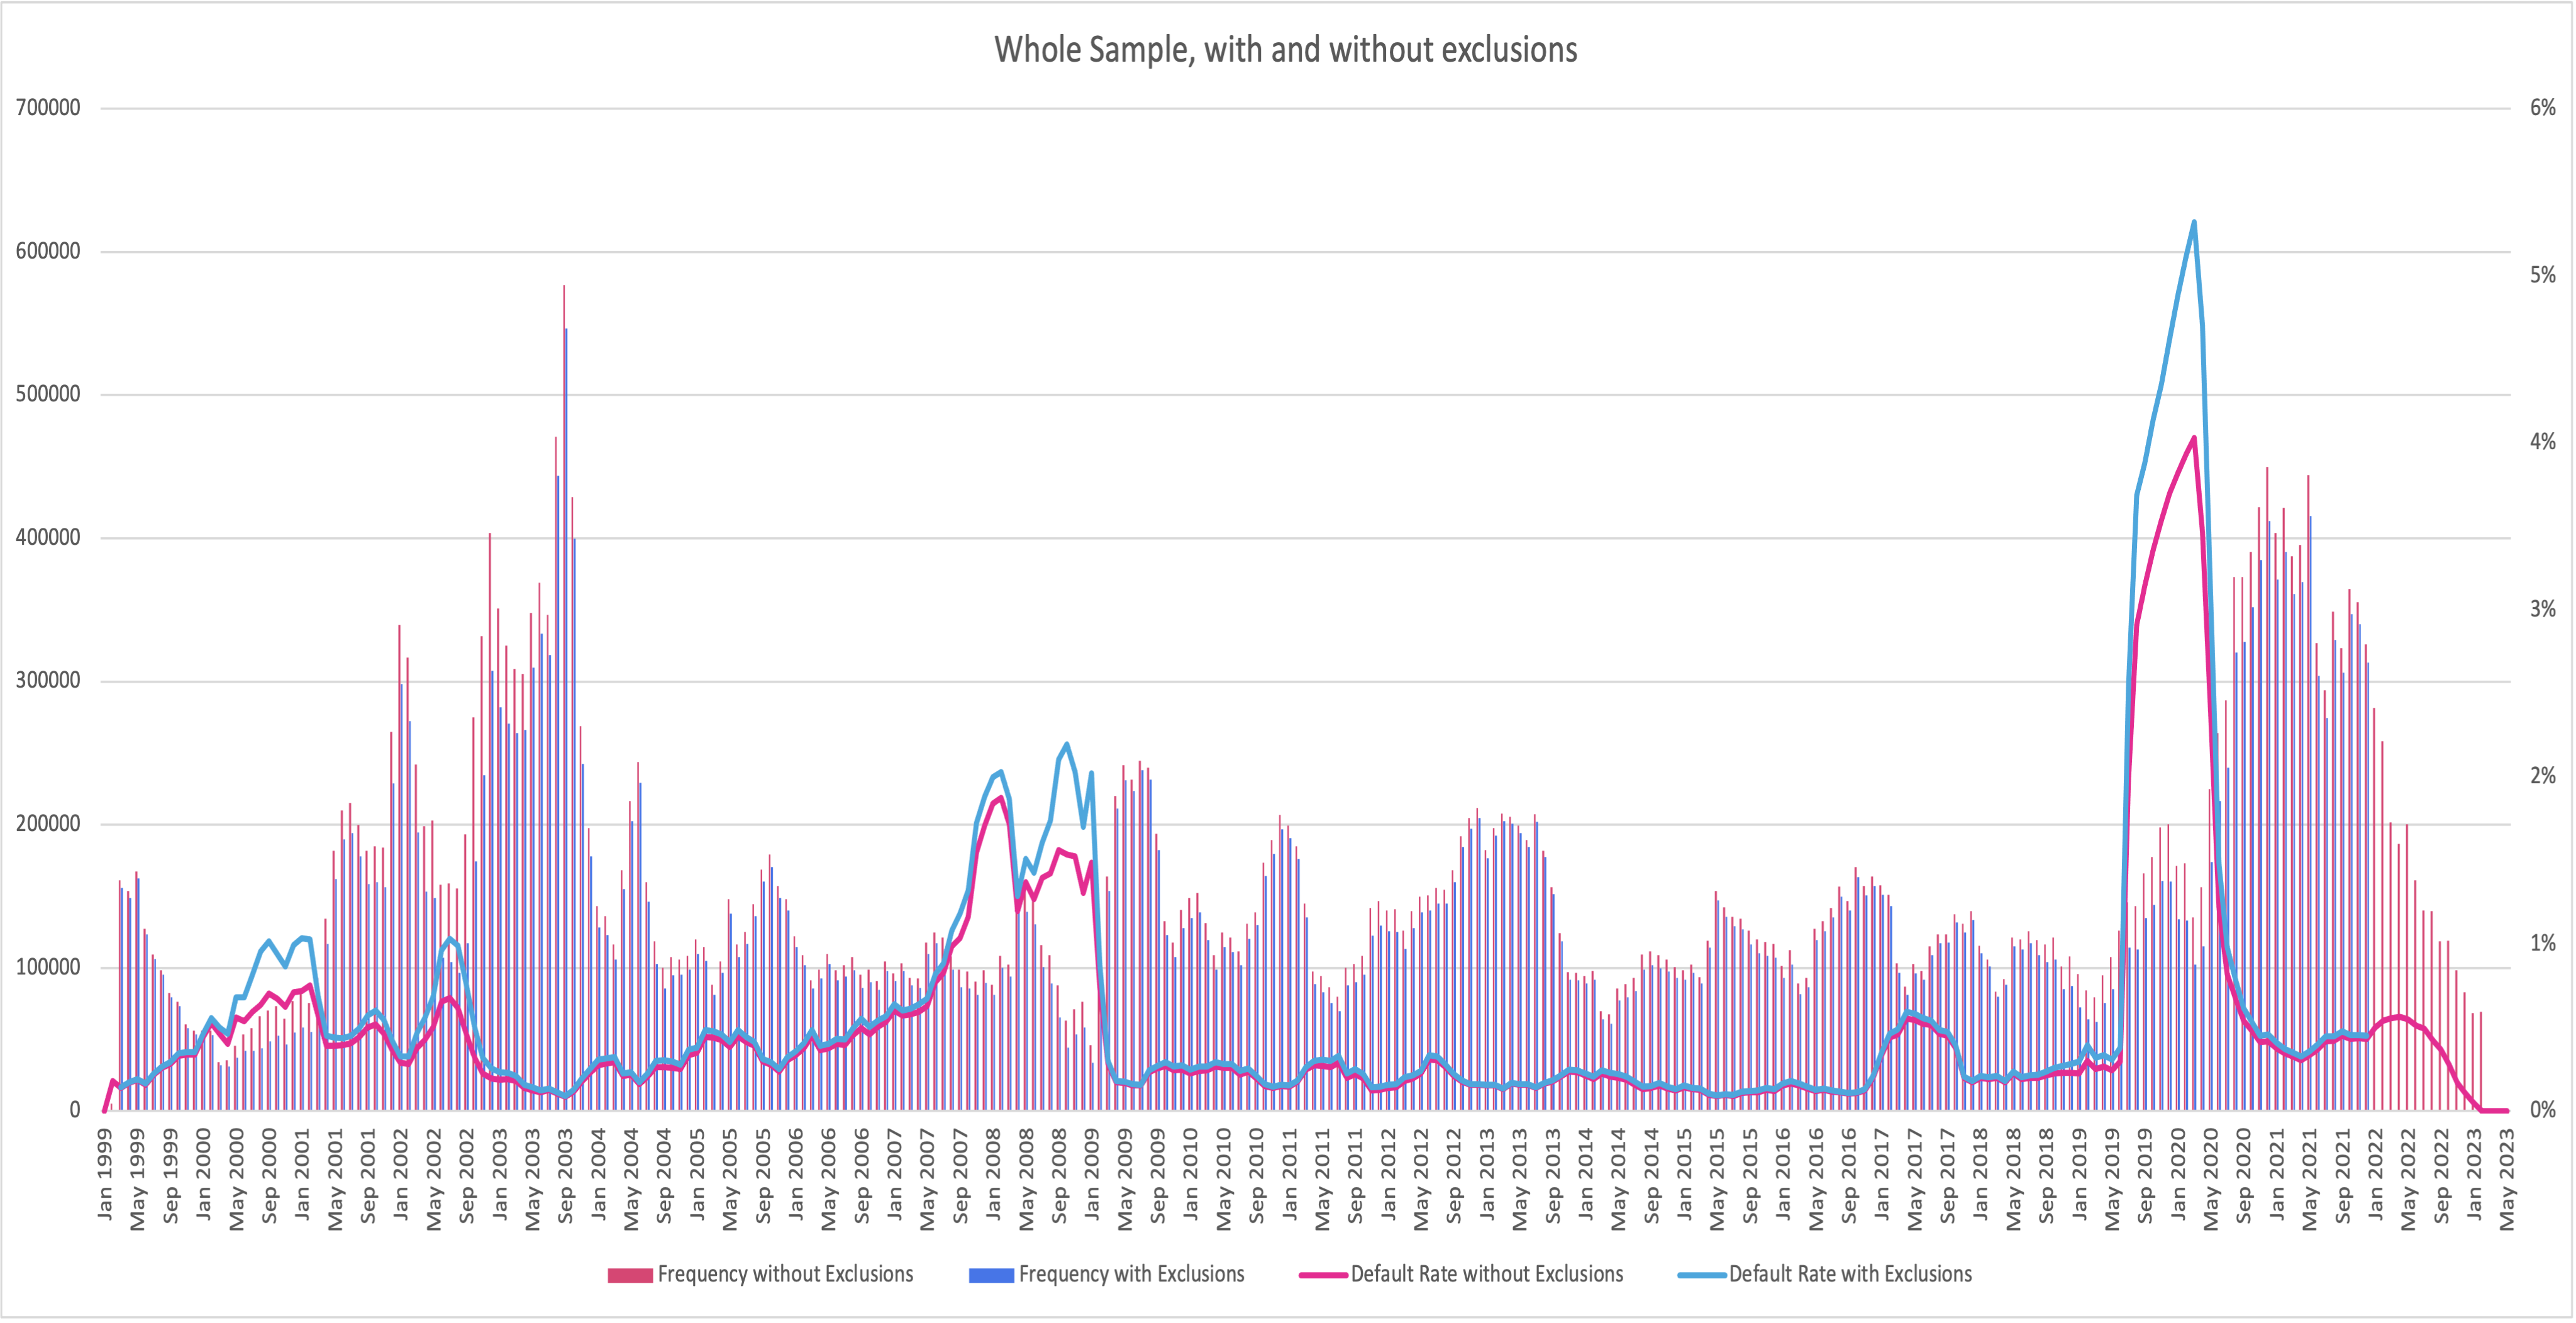
\includegraphics[width=\textwidth]{./FullSample.png}
    \caption{Distribution and default rate of whole sample}
    \label{fig:re_wholesample}
\end{figure}
\begin{figure}[H]
	\centering
	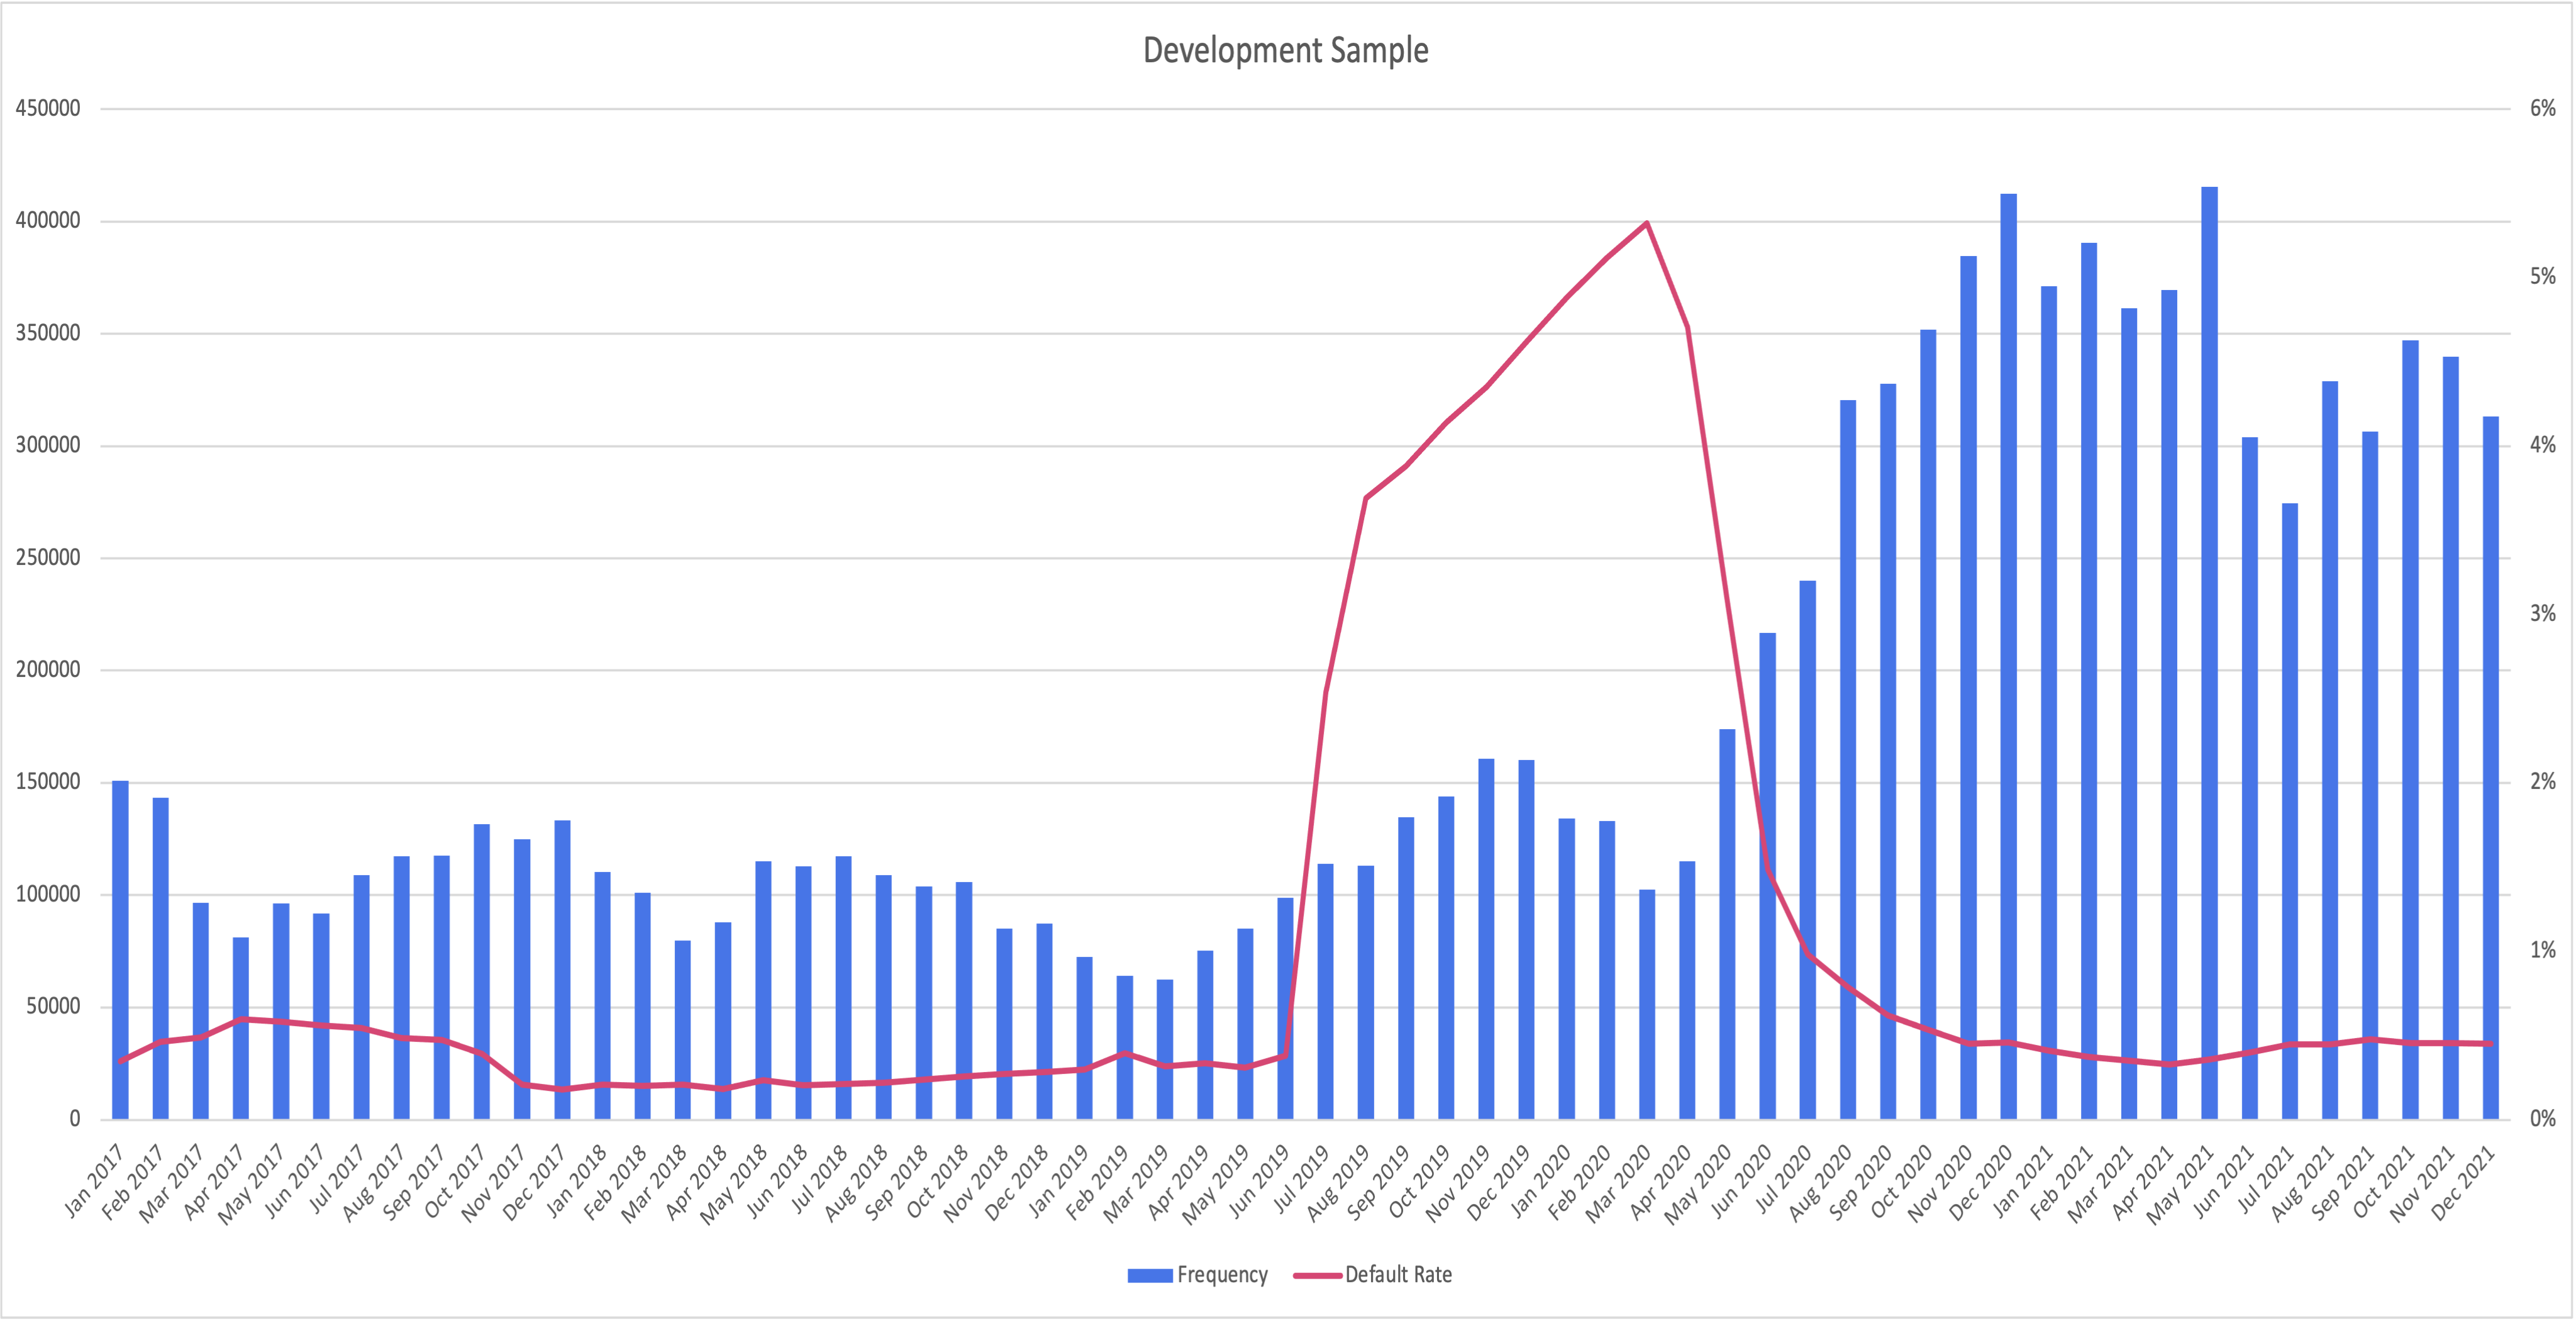
\includegraphics[width=\textwidth]{./DevelopmentSample.png}
    \caption{Distribution and default rate of development sample}
    \label{fig:re_devsample}
\end{figure}

\section{Data preparation}
\subsection{Missing and Erroneous Data Treatment}
The variables were first split into three types: categorical, indicator/binary and numerical variables. The missing rate of all variables were determined and are given in table \ref{tab:re_discr_power}. Program Indicator, HARP Indicator and Super Conforming Flag show a very high missing value proportion of over 90\% and are therefore no candidates for the model. All other risk factors either don't have missing values or an acceptable amount of less than 20\%. Due to the low number of missing values for the numerical variables DTI, Credit Score and other numerical variables with a missing rate below the 3rd decimal, simply the median was imputed (seen in table \ref{tab:re_descr_stat}). For Property Valuation Method and other categorical risk factors, these data points were analysed as a separate category. Missing values of indicator variables were set to = 'Y'. 

A treatment of erroneous data was not performed, because data entries outside of pre-defined ranges were already set as "Not Available" or "999" by Freddie Mac and therefore, additional analysis of possible error was not considered necessary. 

\subsection{Outlier Treatment}
The outliers were detected using the interquartile approach explained in chapter XX and visually presented by creating boxplots, visible in Fig. XX - YY. The upper and lower boarders were therefore calculated using the forumals \ref{eq:dp_iqr_boxpl2} and \ref{eq:dp_iqr_boxpl2}. The quartiles of all numerical risk factors are displayed in table \ref{tab:re_descr_stat} and the resulting limits are visible in table \ref{tab:re_iqr}. The proportion of upper and lower outliers were calculated to analyse, if a significant amount of data entries are affected and could influence the modelling process. All variable show outliers - however, only the variables Mortgage Insurance Percentage and Original Loan Term show a concerning amount. New risk factors were derived to circumvent this issue. Multiple versions of indicator variables were created using the definition listed in table \ref{tab:re_descr_newvar}. Additionally, after analysing the distribution and box plots of LTV and CLTV and considering, that they are ratios, a winsorization was performed on both variables to test, if the outliers affect the modelling process negatively. Therefore, data points with values above the upper or below the lower limit, were capped at the respective limit. 

% Please add the following required packages to your document preamble:
% \usepackage{graphicx}
% \usepackage{lscape}
\begin{landscape}

\begin{table}[]
\centering
\resizebox{1.3\textwidth}{!}{%
\begin{tabular}{llllllllllllll}\toprule
\textbf{Variable}     & \textbf{Sum}               & \textbf{Mean}    & \textbf{Mode}    & \textbf{StdDev}  & \textbf{Min}   & \textbf{P1}     & \textbf{P5}     & \textbf{P25}     & \textbf{Median}  & \textbf{P75}     & \textbf{P95}     & \textbf{P99}     & \textbf{Max}       \\\midrule
CLTV         & 789.276.016       & 72      & 80      & 18      & 2     & 24     & 38     & 61      & 75      & 83      & 95      & 97      & 645       \\
No Borrowers & 16.196.343        & 1       & 1       & 1       & 1     & 1      & 1      & 1       & 1       & 2       & 2       & 2       & 6         \\
No Units     & 11.234.497        & 1       & 1       & 0       & 1     & 1      & 1      & 1       & 1       & 1       & 1       & 2       & 4         \\
DTI          & 370.260.245       & 34      & 45      & 10      & 1     & 12     & 17     & 27      & 35      & 42      & 48      & 50      & 65        \\
Credit Score & 8.221.074.894     & 752     & 801     & 44      & 300   & 636    & 669    & 722     & 761     & 789     & 809     & 817     & 850       \\
LTV          & 786.544.248       & 72      & 80      & 18      & 2     & 24     & 38     & 60      & 75      & 82      & 95      & 97      & 611       \\
MI Perc      & 67.423.997        & 6       & -       & 11      & -     & -      & -      & -       & -       & 6       & 30      & 30      & 55        \\
Loan Term    & 3.513.344.140     & 321     & 360     & 72      & 60    & 156    & 180    & 360     & 360     & 360     & 360     & 360     & 506       \\
UPB          & 2.905.914.537.000 & 265.889 & 200.000 & 137.670 & 6.000 & 56.000 & 88.000 & 162.000 & 240.000 & 346.000 & 518.000 & 689.000 & 1.582.000 \\\bottomrule
\end{tabular}%
}
\caption{Descriptive statistics}
\label{tab:re_descr_stat}
\end{table}

\begin{table}[]
\centering
\resizebox{1.3\textwidth}{!}{%
\begin{tabular}{lrrrrrrrr}\toprule
\textbf{Variable} & \textbf{Lower Boarder}     & \textbf{Upper Boarder} & \textbf{\# below Lower Boarder} & \textbf{\# above Upper Boarder} & \textbf{\% below Lower Boarder} & \textbf{\% above Upper Boarder} & \textbf{\# Outliers} & \textbf{\% Outliers} \\\midrule
CLTV              & 28                                             & 116                                        & 181.953                                             & 2.922                                               & 1,66\%                                              & 0,03\%                                              & 184.875                                  & 1,69\%                                   \\
No Borrowers      & -                                            1 & 4                                          & 1                                                   & 9.409                                               & 0,00\%                                              & 0,09\%                                              & 9.410                                    & 0,09\%                                   \\
No Units          & 1                                              & 1                                          & -                                                   & 218.561                                             & 0,00\%                                              & 2,00\%                                              & 218.561                                  & 2,00\%                                   \\
DTI               & 5                                              & 65                                         & 77.087                                              & 20                                                  & 0,71\%                                              & 0,00\%                                              & 77.107                                   & 0,71\%                                   \\
Credit Score      & 622                                            & 890                                        & 24.181                                              & -                                                   & 0,22\%                                              & 0,00\%                                              & 24.181                                   & 0,22\%                                   \\
LTV               & 27                                             & 115                                        & 164.222                                             & 2.015                                               & 1,50\%                                              & 0,02\%                                              & 166.237                                  & 1,52\%                                   \\
MI Perc           & -                                            9 & 15                                         & 21                                                  & 2.252.233                                           & 0,00\%                                              & 20,61\%                                             & 2.252.254                                & 20,61\%                                  \\
Loan Term         & 360                                            & 360                                        & 2.628.031                                           & 45                                                  & 24,05\%                                             & 0,00\%                                              & 2.628.076                                & 24,05\%                                  \\
UPB               & -                           114.000            & 622.000                                    & -                                                   & 203.564                                             & 0,00\%                                              & 1,86\%                                              & 203.564                                  & 1,86\%  \\\bottomrule                                
\end{tabular}%
}
\caption{Interquartile range}
\label{tab:re_iqr}
\end{table}

\end{landscape}

\section{Variable Selection}
\subsection{Univariate Analysis}

\subsubsection{New variables}
During the Outlier Treatment, a few new variables were created. While analysing the different distinct values of categorical variables, risk factor Property states was grouped to five US regions according to their geographical position: Northeast,  outheast, Southwest, Midwest, West and other Regions, e.g. outside of the North American  continent. A summary of the new variables is listed in table \ref{tab:re_descr_newvar}.

\begin{table}[h!]
\centering
\begin{tabular}{ Lp{8cm}R } \toprule
\textbf{Variable Name}  & \textbf{Description}                                                                                                                                                                                                                                                          & \textbf{Abbr.}       \\\midrule
MI Percentage Indicator                                        & Indicator, that Mortgage Insurance Percentage \textgreater 0\%                           & MI Flag                     \\\hline
Loan Term \textgreater 360 Months                              & Indicator, that Original Loan Term \textgreater 360 Months                               & Loan Term \textgreater 360m \\\hline
Loan Term Group                                                & Grouped Variable, Original Loan Term is "\textless 360m", "= 360m", "\textgreater{}360m" & Loan Term Group             \\\hline
Loan Term $\geq$ 360 Months Indicator                          & Indicator, that Original Loan Term $\geq$ 360 Months                                     & Loan Term $\geq$ 360m        \\\hline
Indicator, that Original Loan Term = 360 Months                & Indicator, that Original Loan Term = 360 Months                                          & Loan Term = 360m            \\\hline
Original Combined Loan-to-Value (CLTV) after Outlier Treatment & Original Combined Loan-to-Value (CLTV) after Outlier Treatment                           & CLTV adj                    \\\hline
Original Loan-to-Value (LTV) after Outlier Treatment           & Original Loan-to-Value (LTV) after Outlier Treatment                                     & LTV adj                     \\\hline
US Region                                                      & Grouped variable of "Property State"                                                     & US Region                \\\bottomrule
\end{tabular}%
\caption{Description of new variables}
\label{tab:re_descr_newvar}
\end{table}

\subsubsection{Discriminatory power}
To assess the discriminatory power, the distribution plots including the default rates and ROC-curves were created as well as AUC and GINI coefficients were calculated. A full list of all metrics is given in table \ref{tab:re_discr_power} and plots of relevant variables are given in Fig. XX to Fig. YY. All plots are displayed in Annex xx. As expected, the external credit score provided by FICO shows the highest discriminatory power, followed by financial ratios, e.g., DTI, LTV and CLTV. Other numerical risk factors indicate good predictive power and were therefore seen as candidates for the modelling process, but instead of the raw variable, the indicator version Loan Term $\geq$ 360m and MI Flag were selected. The performance of the categorical and indicator risk factors were disappointing, with barely any GINI coefficients above 5\%. A Gini threshold of 5\% was therefore set for the selection process of the long list. 

To summarize, all variables with a missing proportion below 20\%, outlier proportion not succeeding 20\% and GINI coefficient above 5\% were selected for the long list given in table \ref{tab:re_ll_sl}. 

\newpage
\begin{longtable}{ l p{5.5cm} l l l }\toprule      
\textbf{Variable}           & \textbf{Value}                                     & \textbf{\% Missing} & \textbf{GINI}    & \textbf{AUC}    \\\midrule
Amort Type                  & Fixed Rate Mortgage                                & 0,00\%     & 0,00\%  & 0,5000 \\\hline
Prop Val Method             & ACE Loans                                          & 2,78\%     & 9,80\%  & 0,5490 \\
                            & Full Appraisal                                     & 2,78\%     & 11,74\% & 0,5587 \\
                            & Other Appraisals (Desktop, driveby, external, AVM) & 2,78\%     & 0,33\%  & 0,5017 \\
                            & Not Available                                      & 2,78\%     & 1,61\%  & 0,5081 \\\hline
Channel                     & Not Available                                      & 0,00\%     & 0,00\%  & 0,5000 \\
                            & Broker                                             & 0,00\%     & 1,05\%  & 0,5052 \\
                            & Correspondent                                      & 0,00\%     & 7,21\%  & 0,5361 \\
                            & Retail                                             & 0,00\%     & 8,26\%  & 0,5413 \\
                            & TPO Not Specified                                  & 0,00\%     & 0,00\%  & 0,5000 \\\hline
Prog Flag                   & Not Available or Not Applicable                    & 94,03\%    & 4,56\%  & 0,5228 \\
                            & HFA Advantage                                      & 94,03\%    & 0,78\%  & 0,5039 \\
                            & Home Possible                                      & 94,03\%    & 3,78\%  & 0,5189 \\
                            & Refi Possible                                      & 94,03\%    & 0,00\%  & 0,5000 \\\hline
Loan Purpose                & Refinance - Cash Out                               & 0,00\%     & 1,05\%  & 0,5053 \\
                            & Refinance - No Cash Out                            & 0,00\%     & 5,26\%  & 0,5263 \\
                            & Purchase                                           & 0,00\%     & 4,21\%  & 0,5210 \\\hline
Occupancy                   & Investment Property                                & 0,00\%     & 0,20\%  & 0,5010 \\
                            & Primary Residence                                  & 0,00\%     & 1,00\%  & 0,5050 \\
                            & Second Home                                        & 0,00\%     & 1,20\%  & 0,5060 \\\hline
Loan Term Group             & = 360 Months                                       & 0,00\%     & 10,23\% & 0,5512 \\
                            & \textgreater{}. 360 Months                         & 0,00\%     & 0,01\%  & 0,5000 \\
                            & \textless 360 Months                               & 0,00\%     & 10,24\% & 0,5512 \\\hline
Prop Type                   & Condo                                              & 0,00\%     & 0,34\%  & 0,5017 \\
                            & Co-op                                              & 0,00\%     & 0,04\%  & 0,5002 \\
                            & Manufactured Housing                               & 0,00\%     & 0,04\%  & 0,5002 \\
                            & PUD                                                & 0,00\%     & 0,53\%  & 0,5026 \\
                            & Single-Family                                      & 0,00\%     & 0,79\%  & 0,5039 \\\hline
US Region                   & Midwest                                            & 0,00\%     & 5,92\%  & 0,5296 \\
                            & Northeast                                          & 0,00\%     & 1,79\%  & 0,5090 \\
                            & Other                                              & 0,00\%     & 0,06\%  & 0,5003 \\
                            & South                                              & 0,00\%     & 3,00\%  & 0,5150 \\
                            & West                                               & 0,00\%     & 1,07\%  & 0,5054 \\\midrule
Homebuyer Flag              &                                                    & 0,00\%     & 5,15\%  & 0,5258 \\
Int Only Flag               &                                                    & 0,00\%     & 0,00\%  & 0,5000 \\
MI Flag                     &                                                    & 0,00\%     & 12,93\% & 0,5647 \\
Loan Term = 360m            &                                                    & 0,00\%     & 10,23\% & 0,5512 \\
Loan Term $\geq$ 360m       &                                                    & 0,00\%     & 10,24\% & 0,5512 \\
Loan Term \textgreater 360m &                                                    & 0,00\%     & 0,01\%  & 0,5000 \\
Sup Conf Flag               &                                                    & 96,26\%    & 0,00\%  & 0,5000 \\
HARP Flag                   &                                                    & 99,35\%    & 0,00\%  & 0,5000 \\
PPM Flag                    &                                                    & 0,00\%     & 0,00\%  & 0,5000 \\\midrule
CLTV                        &                                                    & 0,00\%     & 21,04\% & 0,6052 \\
No Borrowers                &                                                    & 0,00\%     & 11,33\% & 0,5566 \\
No Units                    &                                                    & 0,00\%     & 1,27\%  & 0,5064 \\
DTI                         &                                                    & 0,66\%     & 26,60\% & 0,6330 \\
Credit Score                &                                                    & 0,02\%     & 34,58\% & 0,6729 \\
LTV                         &                                                    & 0,00\%     & 20,75\% & 0,6038 \\
MI Perc                     &                                                    & 0,00\%     & 13,14\% & 0,5657 \\
Loan Term                   &                                                    & 0,00\%     & 10,51\% & 0,5526 \\
UPB                         &                                                    & 0,00\%     & 10,44\% & 0,5522 \\\bottomrule
    
\caption{Discriminatory power}
\label{tab:re_discr_power}           
\end{longtable}

\subsection{Multivariate Analysis}

The shortlist was created using the following process: First, the correlation matrix with all numerical variables was created. Then, the variable with the highest GINI coefficient was selected and all risk factors with a correlation coefficient above +0.25 or below -0.25 are removed. This step should be repeated with the remaining variables until all features were analysed. 
Table \ref{tab:re_corr_matrix} shows the correlation coefficient for all numeric variables in the long list. Possible interaction effects between categorical and indicator variables are considered using the Variance blabla (VIF) during the modelling process. A correlation coefficient of 100\% between the original and winsorized version of ltv and ctlv is expected as well as a coefficient of 99\% between cltv and ltv. Because the CLTV without outlier treatment shows the highest discriminatory power, all other correlated variables were not considered for the modelling process. The short list is given in table \ref{tab:re_ll_sl}.

\begin{table}[h!]
\resizebox{\textwidth}{!}{%
\begin{tabular}{ llllllll }\toprule    
\textbf{Variable}     & \textbf{Credit Score} & \textbf{CLTV}  & \textbf{CLTV adj} & \textbf{DTI}   & \textbf{LTV}   & \textbf{LTV adj} & \textbf{No Borrowers} \\\midrule
Credit Score & 1            & -0,11 & -0,11    & -0,17 & -0,11 & -0,11   & -0,05        \\
CLTV         & -0,11        & 1     & 1        & 0,12  & 0,99  & 0,99    & -0,06        \\
CLTV adj     & -0,11        & 1     & 1        & 0,12  & 0,99  & 0,99    & -0,06        \\
DTI          & -0,17        & 0,12  & 0,12     & 1     & 0,12  & 0,12    & -0,08        \\
LTV          & -0,11        & 0,99  & 0,99     & 0,12  & 1     & 1       & -0,06        \\
LTV adj      & -0,11        & 0,99  & 0,99     & 0,12  & 1     & 1       & -0,06        \\
No Borrowers & -0,05        & -0,06 & -0,06    & -0,08 & -0,06 & -0,06   & 1           \\\bottomrule
\end{tabular}%
}
\caption{Correlation matrix}
\label{tab:re_corr_matrix}   
\end{table}

\begin{longtable}{ l p{5.5cm} p{5.5cm} }\toprule    
\textbf{Variable}                    & \textbf{Long List}                                                                                                          & \textbf{Short List}                                                                                              \\\midrule
Credit Score                & \cellcolor[HTML]{B4EDB3}Missing Treatment applied                                                             & \cellcolor[HTML]{B4EDB3}                                                                           \\
Homebuyer Flag              & \cellcolor[HTML]{B4EDB3}Missing Treatment applied                                                             & \cellcolor[HTML]{B4EDB3}                                                                           \\
MI Perc                     & \cellcolor[HTML]{EDA8A0}Adapted Variable derived (MI Flag)                                                    & -                                                                                                  \\
No Units                    & \cellcolor[HTML]{EDA8A0}Low GINI                                                                              & -                                                                                                  \\
Occupancy                   & \cellcolor[HTML]{EDA8A0}Low GINI                                                                              & -                                                                                                  \\
CLTV                        & \cellcolor[HTML]{B4EDB3}Missing Treatment applied, additional Variable derived with Outlier Treatment applied & \cellcolor[HTML]{B4EDB3}Variable without Outlier Treatment used due to higher discriminatory power \\
DTI                         & \cellcolor[HTML]{B4EDB3}Missing Treatment applied                                                             & \cellcolor[HTML]{B4EDB3}                                                                           \\
UPB                         & \cellcolor[HTML]{B4EDB3}Missing Treatment applied                                                             & \cellcolor[HTML]{B4EDB3}                                                                           \\
LTV                         & \cellcolor[HTML]{B4EDB3}Missing Treatment applied, additional Variable derived with Outlier Treatment applied & \cellcolor[HTML]{EDA8A0}Correlated with CLTV                                                       \\
Channel                     & \cellcolor[HTML]{B4EDB3}                                                                                      & \cellcolor[HTML]{B4EDB3}                                                                           \\
PPM Flag                    & \cellcolor[HTML]{EDA8A0}Low GINI                                                                              & -                                                                                                  \\
Amort Type                  & \cellcolor[HTML]{EDA8A0}Low GINI                                                                              & -                                                                                                  \\
State                       & \cellcolor[HTML]{EDA8A0}Adapted Variable derived (US-region)                                                  & -                                                                                                  \\
Prop Type                   & \cellcolor[HTML]{EDA8A0}Low GINI                                                                              & -                                                                                                  \\
Loan Purpose                & \cellcolor[HTML]{B4EDB3}                                                                                      & \cellcolor[HTML]{B4EDB3}                                                                           \\
Loan Term                   & \cellcolor[HTML]{EDA8A0}Adapted Variable derived (Loan Term $\geq$ 360m)                                      & -                                                                                                  \\
No Borrowers                & \cellcolor[HTML]{B4EDB3}Missing Treatment applied                                                             & \cellcolor[HTML]{B4EDB3}                                                                           \\
Sup Conf Flag               & \cellcolor[HTML]{EDA8A0}Low GINI                                                                              & -                                                                                                  \\
Prog Flag                   & \cellcolor[HTML]{EDA8A0}High Missing Rate                                                                     & -                                                                                                  \\
HARP Flag                   & \cellcolor[HTML]{EDA8A0}Low GINI                                                                              & -                                                                                                  \\
Prop Val Method             & \cellcolor[HTML]{B4EDB3}                                                                                      & \cellcolor[HTML]{B4EDB3}                                                                           \\
Int Only Flag               & \cellcolor[HTML]{EDA8A0}Low GINI                                                                              & -                                                                                                  \\
US Region                   & \cellcolor[HTML]{B4EDB3}                                                                                      & \cellcolor[HTML]{B4EDB3}                                                                           \\
MI Flag                     & \cellcolor[HTML]{B4EDB3}                                                                                      & \cellcolor[HTML]{B4EDB3}                                                                           \\
Loan Term \textgreater 360m & \cellcolor[HTML]{EDA8A0}Low GINI                                                                              & -                                                                                                  \\
Loan Term Group             & \cellcolor[HTML]{EDA8A0}Similar Variable used (Loan Term $\geq$ 360m)                                         & -                                                                                                  \\
Loan Term $\geq$ 360m       & \cellcolor[HTML]{B4EDB3}                                                                                      & \cellcolor[HTML]{B4EDB3}                                                                           \\
Loan Term = 360m            & \cellcolor[HTML]{EDA8A0}Similar Variable used (Loan Term $\geq$ 360m)                                         & -                                                                                               \\\bottomrule
\caption{Long list and Short list}
\label{tab:re_ll_sl}       
\end{longtable}

\section{Modelling}
\subsection{Logistic regression}
Using the stepwise selection algorithm, all short list variables were put into the modelling process. The resulting model is seen in table XX. The order of the risk factors indicate the significance in the model. Only the last variable shows a p-value > 0.05. To limit the number of explanatory variables in the model, the AIC and BIC was calculated for each modelling step. The relative change per step was determined and is visible in table XX. A change is visible in step 10 and therefore all other variables were removed. The final model is visible in table YY, the ROC-curve is displayed in Fig. XX and it shows a discriminatory power of GINI = bla.

\subsection{Boosted Decision Trees}
\section{Comparison}